\documentclass[a4paper,10pt]{article}
\usepackage[utf8]{inputenc}
\usepackage{equation}
\usepackage{graphicx}

% Title Page
\title{Cosmic muon angular distribution from CRY}
\author{Raman Sehgal}


\begin{document}
\maketitle{\textbf{How to get $Cos^{2}\theta$ distribution plot from CRY}}\\

%\begin{abstract}
When running the CRY generator we get simulated cosmic particles. Here we want to understand and visualize the angular distribution of cosmic muons. As we know that cosmic muon follow $Cos^{2}\theta$ distribution. But if one want reconstruct this distribution from CRY generated muon then one should the important of angle at which one has placed the detector in the simuation setup. One can get  $Cos^{2}\theta$ distribution only if the muon detectors are placed perpendicular to the direction of motion of muon, but if the detectors are placed at some angle to direction of motion of muon which is happened in most of the case then one has to do the solid angle correction. Out target is to do this exercise using CRY library.

In our simulation we generate the muons using CRY and our muon detectors are placed vertically in Z direction. This means that the detector plane is not along the normal of the motion of muon. So if we just plot the histogram of angle (of muons generated from CRY with) that it makes with vertically down vector $(0.,0.,-1.)$, then it gives us the distribution corresponding to the LHS of equation \ref{normalAngle}

\begin{equation} \label{normalAngle}
   \centering{ \frac{dN}{d\theta} = I_{0} \ cos^{2}\theta \ dA^{'}\ cos(\theta) \ dt  \ 2\pi  \ Sin(\theta)}  
\end{equation}

\begin{figure}[!htb]
\centering{
    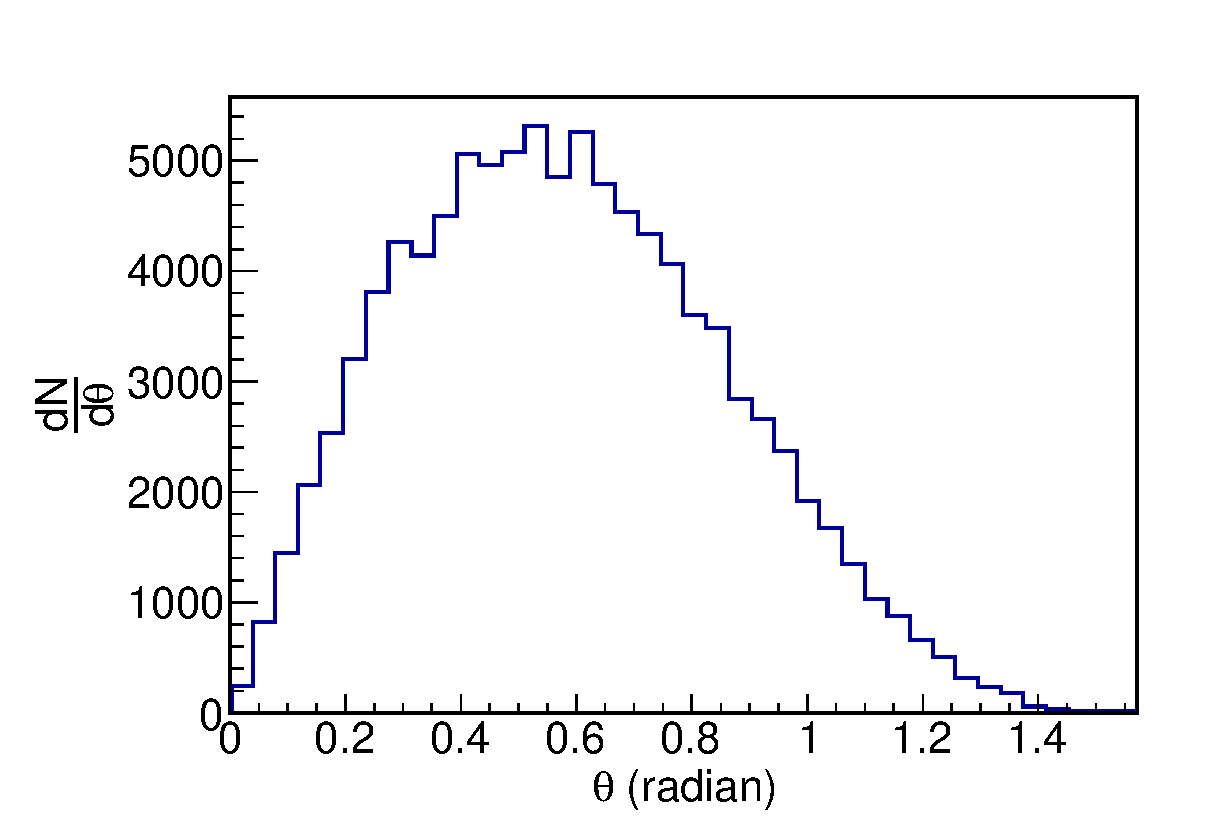
\includegraphics[width=0.55\textwidth]{theta.eps}
    \caption{Angular distribution of muon}
    \label{fig:solidAngles}
    }

\end{figure}

where $dA^{'}$ is very small area element along detector plane. So in order to do the solid angle correction we have to transform this equation to 

\begin{equation}\label{solidAngle}
   \centering{\frac{dN}{dA \ dt \ d\Omega } = I_{0} \ cos^{2}\theta}  
\end{equation}

where $dA = dA^{'}\ cos(\theta)$, i.e area on detector surface is projected along the direction and $d\Omega = 2\pi  \ Sin(\theta) \ d\theta$
   and the fit is done on the LHS of equation \ref{solidAngle}\\

This implies that whatever distribution we get by plotting the histogram of angle of muon w.r.t (0.,0.,-1.) (as shown in figure \ref{fig:solidAngles}), can be converted to $Cos^2{}\theta$, if we divided the bin content of each theta bin by $2\pi \ Sin(\theta) \ Cos(\theta)$, where $\theta$ corresponds to the angle of the bin. In figure \ref{fig:correctedSolidAngles} we can see the the distribution after solid angle correction. To verify the \(cos^2\theta\) distribution, we did the fit using formula \textbf{\(m cos^n\theta\)} in ROOT and found the best fit value of fit parameters \(m = 2.44536 \times 10^3 \pm 13.54\)  is and \(n = 2.025 \pm 0.01666\).

\begin{figure}[!htb]
    \centering{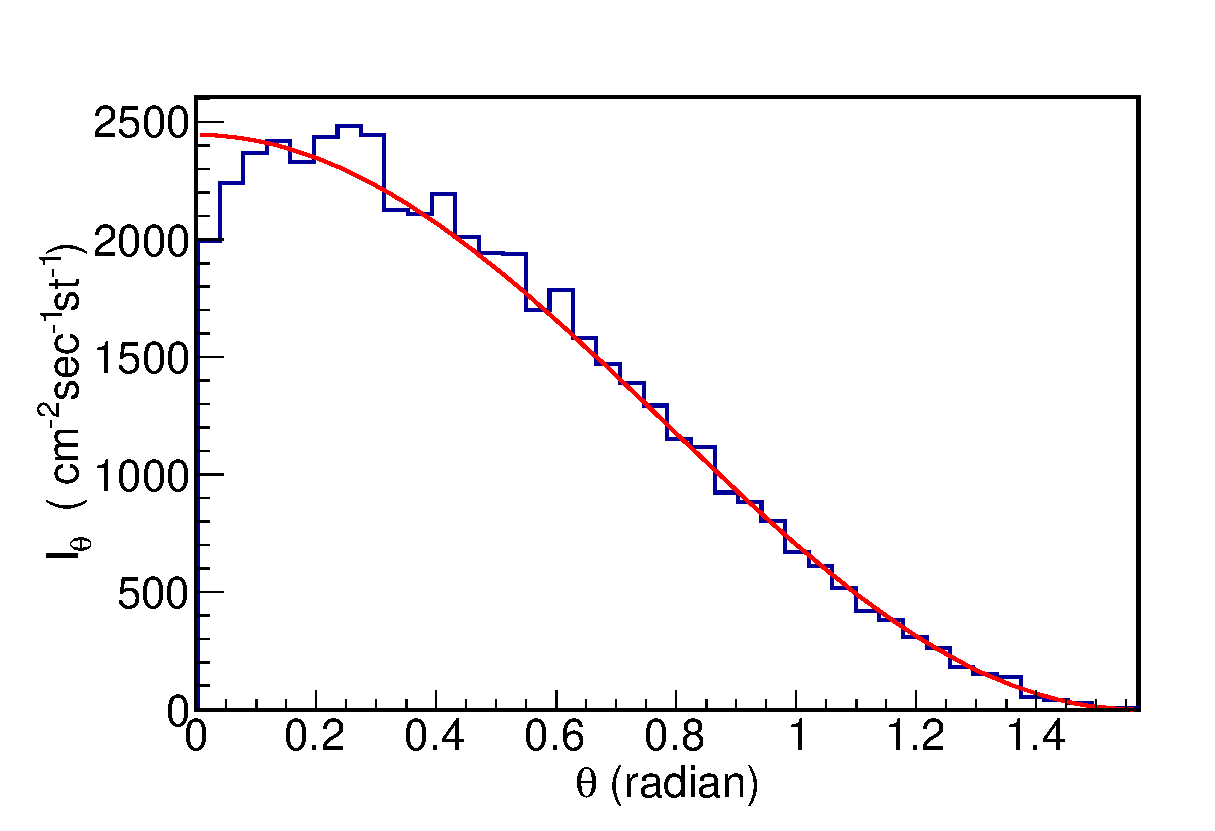
\includegraphics[width=0.55\textwidth]{cos2theta.eps}
    \caption{Solid angle corrected angular distribution of muon}
    \label{fig:correctedSolidAngles}
    }
\end{figure}

%\end{abstract}

\end{document}          
